\documentclass[10pt]{exam}
\usepackage[hon]{template-for-exam}
\usepackage{graphicx}

\title{Range Equation Practice Problems}
\author{Rohrbach}
\date{\today}

\begin{document}
\maketitle

\begin{questions}

  \question
    A projectile is fired with an initial speed of 36.6 m/s at an angle of 42.2 degrees above horizontal on a long flat firing range.  What is the total horizontal distance (that is, range) covered by the projectile?  Compare your answer with question 2(c) on the ``Projectile Motion Practice Problems.''  

    \vs

  \question
    A fire hose held near the ground shoots water at a speed of 6.5~m/s.  Find two angles an which to point the nozzle in order to make the water land 2.5~m away.~\footnote{This problem is adapted from Chapter 3, problem \#23 in Giancolli \textit{Physics with Applications}, 7th ed.}

    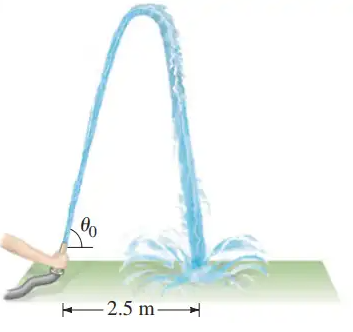
\includegraphics[width=5cm]{hose}

  \vs


  
\end{questions}

\end{document}